\documentclass[10pt, conference]{IEEEtran}
\IEEEoverridecommandlockouts
\usepackage{cite}
\usepackage{amsmath,amssymb,amsfonts}
\usepackage{graphicx}
\usepackage{textcomp}
\usepackage{xcolor}
\usepackage{booktabs}
\usepackage{multirow}
\usepackage{threeparttable}
\usepackage{xfp}

\DeclareMathOperator*{\argmax}{argmax}
\DeclareMathOperator*{\argmin}{argmin}
\newcommand{\etal}{\textit{et al. }}
\newcommand{\red}[1]{\textcolor{red}{#1}}
\newcommand{\blue}[1]{\textcolor{blue}{#1}}


\def\BibTeX{{\rm B\kern-.05em{\sc i\kern-.025em b}\kern-.08em
    T\kern-.1667em\lower.7ex\hbox{E}\kern-.125emX}}
\begin{document}

\title{Automated Lightweight RFFI via PCA-Driven Channel Pruning and Self-Distillation}

\author{
\IEEEauthorblockN{
Keyi~Mo\IEEEauthorrefmark{1},
Guanxiong~Shen\IEEEauthorrefmark{1}\IEEEauthorrefmark{2}
}

\IEEEauthorblockA{
\IEEEauthorrefmark{1}
School of Cyber Science and Engineering, Southeast University, Nanjing, China
}
\IEEEauthorblockA{
\IEEEauthorrefmark{2}
Corresponding Author
}

}

\maketitle


\begin{abstract}
Radio frequency fingerprint identification (RFFI) has emerged as a promising physical-layer authentication technique that exploits device-specific hardware impairments embedded in transmitted radio signals.
Recent RFFI systems increasingly rely on deep neural networks for feature extraction and identification, achieving strong performance under diverse channel conditions.
However, the computational complexity and memory footprint of such models severely limit their real-time execution and direct deployment on resource-constrained edge devices.
Existing lightweight approaches rely on manually designed compact architectures or heuristic channel pruning, where the degree of compression is determined by human intuition rather than the intrinsic properties of learned representations.
This paper presents an automated lightweight RFFI pipeline that derives compact network architectures directly from trained models through PCA-driven channel diagnosis.
We first train a high-capacity teacher network to establish a discriminative RF fingerprint embedding space.
Principal component analysis is then applied to the output feature maps of every convolutional layer, revealing the effective channel dimension required to preserve 95\% of the cumulative variance.
A compact student network is constructed by replacing each layer's channel count with its PCA-derived effective dimension, with weights fully randomly reinitialized.
Self-distillation transfers the teacher's knowledge to the student via temperature-scaled KL divergence in a shared PCA-aligned low-dimensional subspace.
An optional iterative mode chains successive rounds of diagnosis, pruning, and distillation for accuracy-bounded progressive compression.
Experiments across five diverse architectures on a real-world LoRa dataset demonstrate 14--834$\times$ parameter compression with minimal accuracy degradation, and show that self-distillation can even purify representations when the teacher is undertrained, with the student consistently outperforming its teacher.
\end{abstract}


\begin{IEEEkeywords}
Physical layer security, radio frequency fingerprinting, model compression, principal component analysis, knowledge distillation.
\end{IEEEkeywords}


\section{Introduction}
Radio frequency fingerprint identification (RFFI) has emerged as a compelling physical-layer (PHY) authentication mechanism for Internet of Things (IoT) systems, exploiting unique hardware-inherent imperfections to secure resource-constrained devices where traditional cryptography is impractical. 
To guarantee seamless communication without introducing protocol blockages, modern RFFI deployments strictly require real-time, per-packet local verification with sub-millisecond inference latency on edge platforms.
While deep convolutional and residual networks have delivered remarkable authentication accuracy and channel robustness, they predominantly rely on over-parameterized architectures. 
Their prohibitive computational budgets and memory footprints fundamentally contradict the rigid latency and energy constraints of edge hardware, motivating an urgent need for structural model compression.

However, existing lightweight RFFI methodologies fail to balance efficiency and classification accuracy due to their reliance on human-crafted heuristics. 
Conventional approaches typically enforce a uniform width multiplier across all convolutional layers or apply hand-picked channel importance criteria. 
These methods share a critical paradigm limitation: the layer-wise compression scaling is dictated by manual intuition rather than the intrinsic characteristics of the learned signal representations. 
In RFFI tasks, physical-layer signal features exhibit severe spatial and layer-wise heterogeneity, making uniform pruning strategies fundamentally sub-optimal.
A critical observation underpins this work: a fully trained high-capacity network inherently encodes its own architectural redundancy, where the empirical channel-wise energy spectrum derived from principal component analysis (PCA) analytically exposes the exact dimensions required to retain dominant representation variance.

To address these limitations, we propose an automated lightweight RFFI framework. At the architectural level, we introduce a data-driven channel pruning mechanism that utilizes per-layer principal component analysis (PCA) on convolutional feature maps to adaptively eliminate structural redundancy based on representation energy. Regarding the training methodology, we implement a self-distillation paradigm, bypassing parameter inheritance via fully randomly reinitialized student networks. To further bridge the structural discrepancy between heterogeneous topologies, we establish an embedding alignment mechanism in a shared low-dimensional subspace derived from the teacher’s manifold. The entire pipeline supports an optional iterative compression mode bounded by a configurable accuracy floor to progressively approach the model's information-theoretic limits. We evaluate our approach across five diverse architectures on a real-world LoRa dataset covering line-of-sight, non-line-of-sight, and mobile scenarios, and demonstrate its sub-millisecond real-time inference effectiveness on NVIDIA Jetson edge platforms.

The main contributions are summarized as follows.
\begin{itemize}
    \item \textbf{PCA-Driven Channel Pruning across Diverse Architectures.}
    We perform per-layer PCA on Conv2d output feature maps, deriving effective channel dimensions that replace heuristic width multipliers with a data-driven criterion. The method is validated across ResNet, SCSKNet, DenseNet, ShuffleNetV2, and LightNet, each supported by a unified prunable builder interface.

    \item \textbf{Self-Distillation via PCA-Aligned KL Divergence.}
    The randomly-initialized compact network is trained solely from teacher soft labels through temperature-scaled KL divergence in a shared PCA subspace. A PCA projection aligns the teacher's high-dimensional embedding with the student's low-dimensional output, enabling direct distribution matching. We further show that distillation acts as a representation purifier: even when the teacher is undertrained, the student can outperform it by learning from the PCA-filtered soft labels.

    \item \textbf{Iterative Compression with Accuracy Guarantee.}
    An iterative mode chains successive rounds of PCA diagnosis, pruning, and distillation, achieving progressive compression until the accuracy drop exceeds a configurable threshold. We demonstrate convergence behavior across three rounds on ResNet, compressing 14.7$\times$ with improved accuracy and reaching 67.2$\times$ cumulative compression after two rounds.
\end{itemize}

\section{Overview of an RF Fingerprinting System}

\begin{figure}[t]
    \centering
    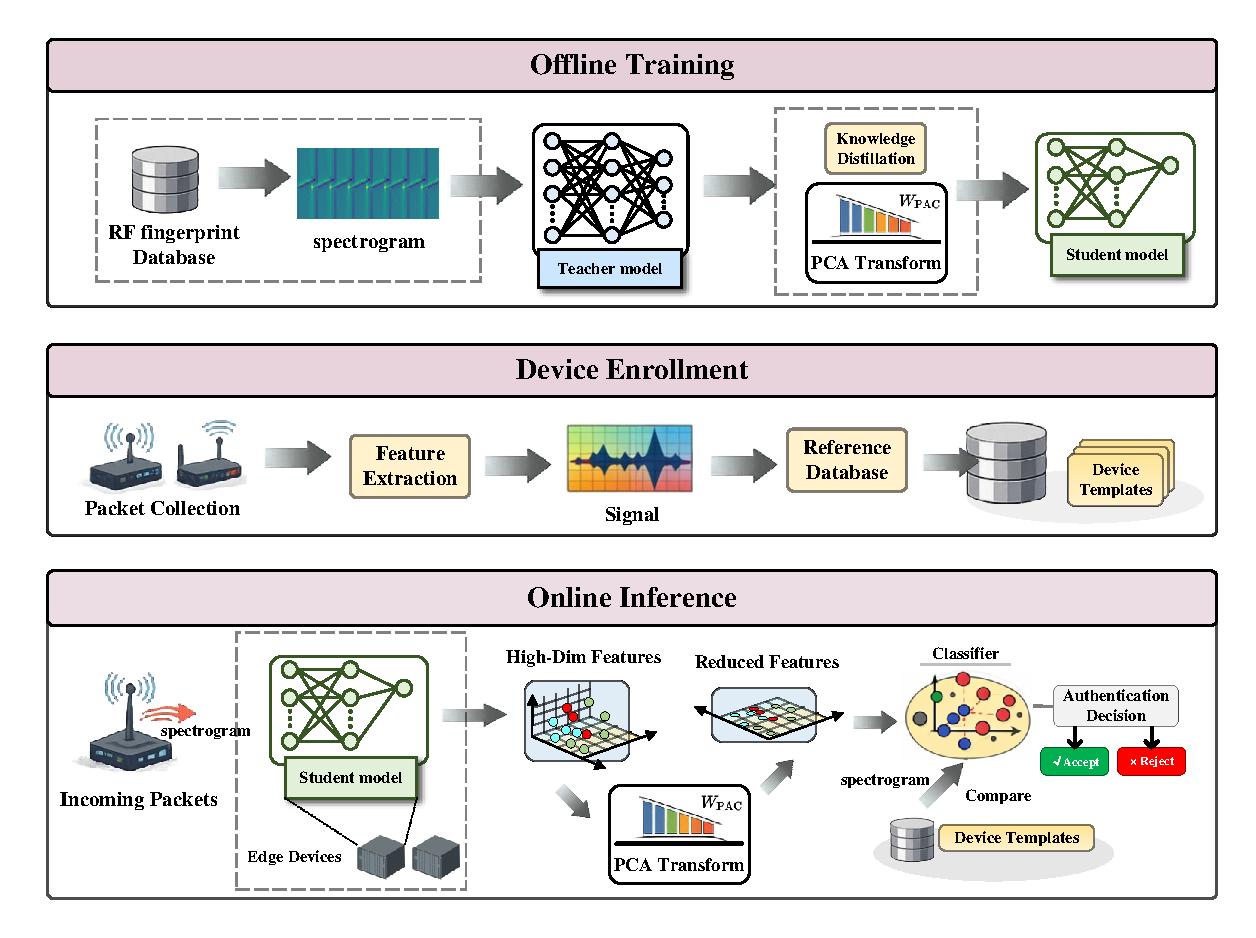
\includegraphics[width=0.95\linewidth]{figures/Overview of an RF Fingerprinting System.pdf}
    \caption{System architecture of the proposed automated lightweight RFFI framework comprising three phases.}
    \label{fig:system_arch}
\end{figure}

This section presents the overall workflow of the proposed automated lightweight RFFI system, which consists of three stages: offline training, device enrollment, and online inference.
Our primary goal is to enable real-time authentication during online inference on edge devices. To this end, the offline training stage is specially optimized as a fully automated four-stage pipeline.

In the offline training stage, a high-capacity teacher network is first trained on a large-scale RF dataset to establish a discriminative embedding space using triplet metric loss.
PCA channel diagnosis is then performed on every convolutional layer of the trained teacher, revealing the effective channel dimension required at each layer.
A compact student network is constructed by replacing each layer's channel count with its PCA-derived effective dimension, with weights fully randomly reinitialized.
Self-distillation transfers the teacher's knowledge to the student via temperature-scaled KL divergence in a shared PCA subspace, producing a compact yet highly discriminative network.
This stage is performed once, typically by a third party with sufficient data and computing resources, and does not require real-time execution.

During the enrollment stage, a small number of packets are collected from each authorized device under controlled conditions.
The deployed student network extracts L2-normalized feature embeddings from these packets, which are stored as reference templates in a local database on the edge device.

In the online inference stage, each newly received wireless packet is processed locally in real time.
The student network extracts its RF fingerprint embedding and compares it against the enrolled templates using KNN on Euclidean distance to make an authentication decision, e.g., accepting the packet as legitimate or rejecting it as unknown or spoofed.
This stage achieves low-latency inference suitable for edge deployment.

\section{PCA-Driven Channel Diagnosis and Structural Pruning}

This section presents the core methodology of our automated pipeline: how PCA is used to diagnose per-layer channel redundancy in a trained network, and how the diagnosis results are translated into a compact architecture.

\subsection{Non-Uniform Channel Redundancy in RFFI Networks}

The conventional approach of applying a uniform width multiplier to all convolutional layers implicitly assumes homogeneous redundancy across the network.
In RFFI networks, this assumption does not hold.
Shallow layers learn low-level time-frequency textures that require more channel diversity, while deep layers extract abstract device-specific features that can be highly compressible.
A uniform multiplier aggressive enough to meet edge constraints, cripples information-critical early layers while leaving later layers unnecessarily wide.
Layer-specific, data-driven channel allocation is therefore required.

\subsection{Per-Layer Conv2d PCA Diagnosis}

Given a trained teacher network, we hook every \texttt{Conv2d} layer and collect its output feature maps during a forward pass over the training set.
For a convolutional layer with $C$ output channels producing a tensor $\mathbf{Y} \in \mathbb{R}^{B \times C \times H \times W}$, we reshape it to $\mathbb{R}^{(B\cdot H\cdot W) \times C}$, treating each spatial position as an independent sample in the channel space.
PCA is then performed on this matrix to obtain eigenvalues $\lambda_1 \ge \lambda_2 \ge \dots \ge \lambda_C$.

The cumulative explained variance ratio after $k$ principal components is defined as:
\begin{equation}
\label{eq:cumsum}
\text{cumsum}(k) = \frac{\sum_{i=1}^{k} \lambda_i}{\sum_{i=1}^{C} \lambda_i}.
\end{equation}

The effective dimension at a threshold $\tau$ is:
\begin{equation}
\label{eq:eff_dim}
d_{\text{eff}} = \argmin_k \left\{ \text{cumsum}(k) \geq \tau \right\}.
\end{equation}

Auxiliary convolutions, i.e., shortcut projections, downsample layers, and depthwise convolutions, are automatically filtered out during analysis, as their channel counts are structurally coupled to main-branch dimensions rather than independently compressible.


\section{Self-Distillation via PCA-Aligned Manifolds}

This section describes a training methodology for the randomly-initialized compact network via self-distillation within a PCA-aligned subspace, enabling the pruned student model to recover teacher-level representation discriminability.

\subsection{Teacher Embedding Space Alignment via PCA}

The teacher network produces high-dimensional embeddings, e.g., $\mathbf{z}_t \in \mathbb{R}^{512}$, while the compact student is designed to output low-dimensional embeddings, e.g., $\mathbf{z}_s \in \mathbb{R}^{8}$.
A direct KL divergence between these two spaces is impossible due to the dimensional mismatch.
To address this, we learn a PCA projection from the teacher's embedding space to the student's dimension.

Let $f_t(\cdot;\theta_t)$ denote the frozen teacher feature extractor.
All training samples are passed through the teacher to collect a feature matrix $\mathbf{Z}_{\text{teach}} \in \mathbb{R}^{N \times d_t}$, where $d_t$ is the teacher embedding dimension.
PCA is performed on this matrix to obtain a projection matrix $\mathbf{W} \in \mathbb{R}^{d_t \times d_s}$ formed by the top-$d_s$ eigenvectors, and a mean vector $\boldsymbol{\mu} \in \mathbb{R}^{d_t}$.
The teacher embedding is then projected and $\ell_2$-normalized:
\begin{equation}
\label{eq:proj}
\hat{\mathbf{z}}_t =
\operatorname{Norm}\!\left(
(\mathbf{z}_t - \boldsymbol{\mu}) \, \mathbf{W}
\right),
\end{equation}
where $\operatorname{Norm}(\cdot)$ denotes $\ell_2$ normalization.
Both teacher and student now operate in the same $\mathbb{R}^{d_s}$ space, enabling direct distribution matching.

\subsection{Distillation Objective}

For each triplet $(\mathbf{x}_a, \mathbf{x}_p, \mathbf{x}_n)$, where the anchor and positive samples originate from the same transmitter and the negative sample comes from a different transmitter, the student $f_s(\cdot;\theta_s)$ produces embeddings $(\mathbf{z}_{a,s}, \mathbf{z}_{p,s}, \mathbf{z}_{n,s}) \in \mathbb{R}^{d_s}$.
The frozen teacher produces high-dimensional embeddings which are PCA-projected to $(\hat{\mathbf{z}}_{a,t}, \hat{\mathbf{z}}_{p,t}, \hat{\mathbf{z}}_{n,t}) \in \mathbb{R}^{d_s}$.

The teacher is first trained with the standard triplet margin loss to establish a discriminative embedding space:
\begin{equation}
\label{eq:triplet}
\mathcal{L}_{\text{tri}} =
\max\Bigl(0,
\lVert \mathbf{z}_{a} - \mathbf{z}_{p} \rVert_2^2 -
\lVert \mathbf{z}_{a} - \mathbf{z}_{n} \rVert_2^2 + m
\Bigr),
\end{equation}
where $m$ is a predefined margin. This loss is used only for pre-training the teacher; the student is trained exclusively via distillation.

After the teacher is frozen, the student is trained by minimizing the temperature-scaled KL divergence between the projected teacher embedding distribution and the student embedding distribution.
The distillation loss is summed over the anchor, positive, and negative positions:
\begin{equation}
\label{eq:kd}
\mathcal{L}_{\text{KD}} =
T^2 \sum_{\mathbf{q} \in \{a,p,n\}}
\mathrm{KL}\!\left(
\operatorname{softmax}\!\left(\frac{\hat{\mathbf{z}}_{\mathbf{q},t}}{T}\right)
\;\Big\Vert\;
\operatorname{softmax}\!\left(\frac{\mathbf{z}_{\mathbf{q},s}}{T}\right)
\right),
\end{equation}
where $T$ is the temperature parameter controlling the softness of the target distribution.

\subsection{Warmup and Early Stopping}

Training a randomly-initialized compact network with pure KL distillation presents a cold-start problem: early KL gradients are noisy because the student embedding manifold is initially unstructured.
We employ two mechanisms to ensure stable convergence.
Minimum epoch warmup guarantees the student at least $E_{\min}$ epochs of training before early stopping can activate, ensuring the student embedding space has time to organize under the teacher's guidance.
Early stopping with patience terminates training if the KNN validation accuracy on the embedding space fails to improve for $P$ consecutive epochs after the warmup phase, preventing overfitting.
The best checkpoint by validation accuracy is restored at the end.

\subsection{Iterative Distillation}

The pipeline can iterate: the distilled student becomes the teacher for the next round.
Let $\theta_t^{(r)}$ denote the teacher at round $r$, with $\theta_t^{(1)}$ being the originally trained large network.
For each round:
\begin{enumerate}
    \item PCA channel diagnosis is performed on $\theta_t^{(r)}$;
    \item A further-compressed student is built from the new PCA results, with randomly reinitialized weights;
    \item Self-distillation transfers knowledge from $\theta_t^{(r)}$ to the new student $\theta_s^{(r)}$;
    \item If $\text{Acc}(\theta_t^{(r)}) - \text{Acc}(\theta_s^{(r)}) \le \delta$, set $\theta_t^{(r+1)} \leftarrow \theta_s^{(r)}$ and continue; otherwise terminate.
\end{enumerate}
This yields an accuracy-bounded compression schedule: the pipeline automatically discovers the Pareto frontier of the accuracy--efficiency trade-off without requiring a predefined target parameter count.


\section{Experimental Evaluation}
\label{sec:experimental_evaluation}

\subsection{Experimental Setup}
\label{subsec:experimental_setup}

\subsubsection{Dataset Description}
\label{subsubsec:dataset_description}

Our experiments utilize a large-scale LoRa RF fingerprinting dataset collected from 60 commercial devices, i.e., Pycom LoPy4/FiPy modules, and a USRP N210 SDR receiver~\cite{shen2021towards}.
The training set consists of 800 packets per device from 40 devices, collected in a controlled, stationary line-of-sight (LOS) residential environment.
The test set evaluates the system across diverse scenarios, from ideal to challenging channel conditions: seen devices under static LOS (three locations A, B, C), unseen devices under NLOS conditions (three obstructed locations D, E, F), and mobile scenarios including device movement in a LOS office and a NLOS meeting room.
All signals are preprocessed via short-time Fourier transform (STFT) to produce single-channel spectrograms.

\subsubsection{Experimental Platforms and Hyperparameters}
\label{subsubsec:hyperparameters}

The training process is performed on a high-performance server equipped with an Intel Core i9 CPU and an NVIDIA RTX 4090 GPU running PyTorch 2.0.
To validate edge deployment feasibility, we deploy the trained student models on an NVIDIA Jetson Nano (4~GB).
All teacher and student networks are trained using the Adam optimizer with an initial learning rate of $10^{-3}$ and a batch size of 16--32.
For teacher pre-training, the triplet margin is set to $m = 0.1$.
For distillation, we use temperature $T = 3.0$, PCA channel threshold $\tau = 0.95$, minimum channels $c_{\min} = 2$, and student embedding dimension $d_s = 8$.
Evaluation uses KNN ($k = 5$) on L2-normalized embeddings with a 50/50 enrollment/test split stratified by device label.

\subsubsection{Teacher Model Selection and Validation Dynamics}
During the high-capacity metric exploration phase, the network is evaluated at the end of each epoch using a randomly sampled 10\% subset of the validation dataset. The network maps these validation signal samples into the high-dimensional embedding space, where classification is performed via a KNN voting classifier employing Euclidean distance metrics. The specific epoch that yields the peak classification accuracy is isolated, and this frozen, optimal teacher artifact serves as the exclusive supervisor to guide the manifold alignment and dual-constraint learning of the randomly-initialized compact student network.

\begin{figure}[t]
    \centering
    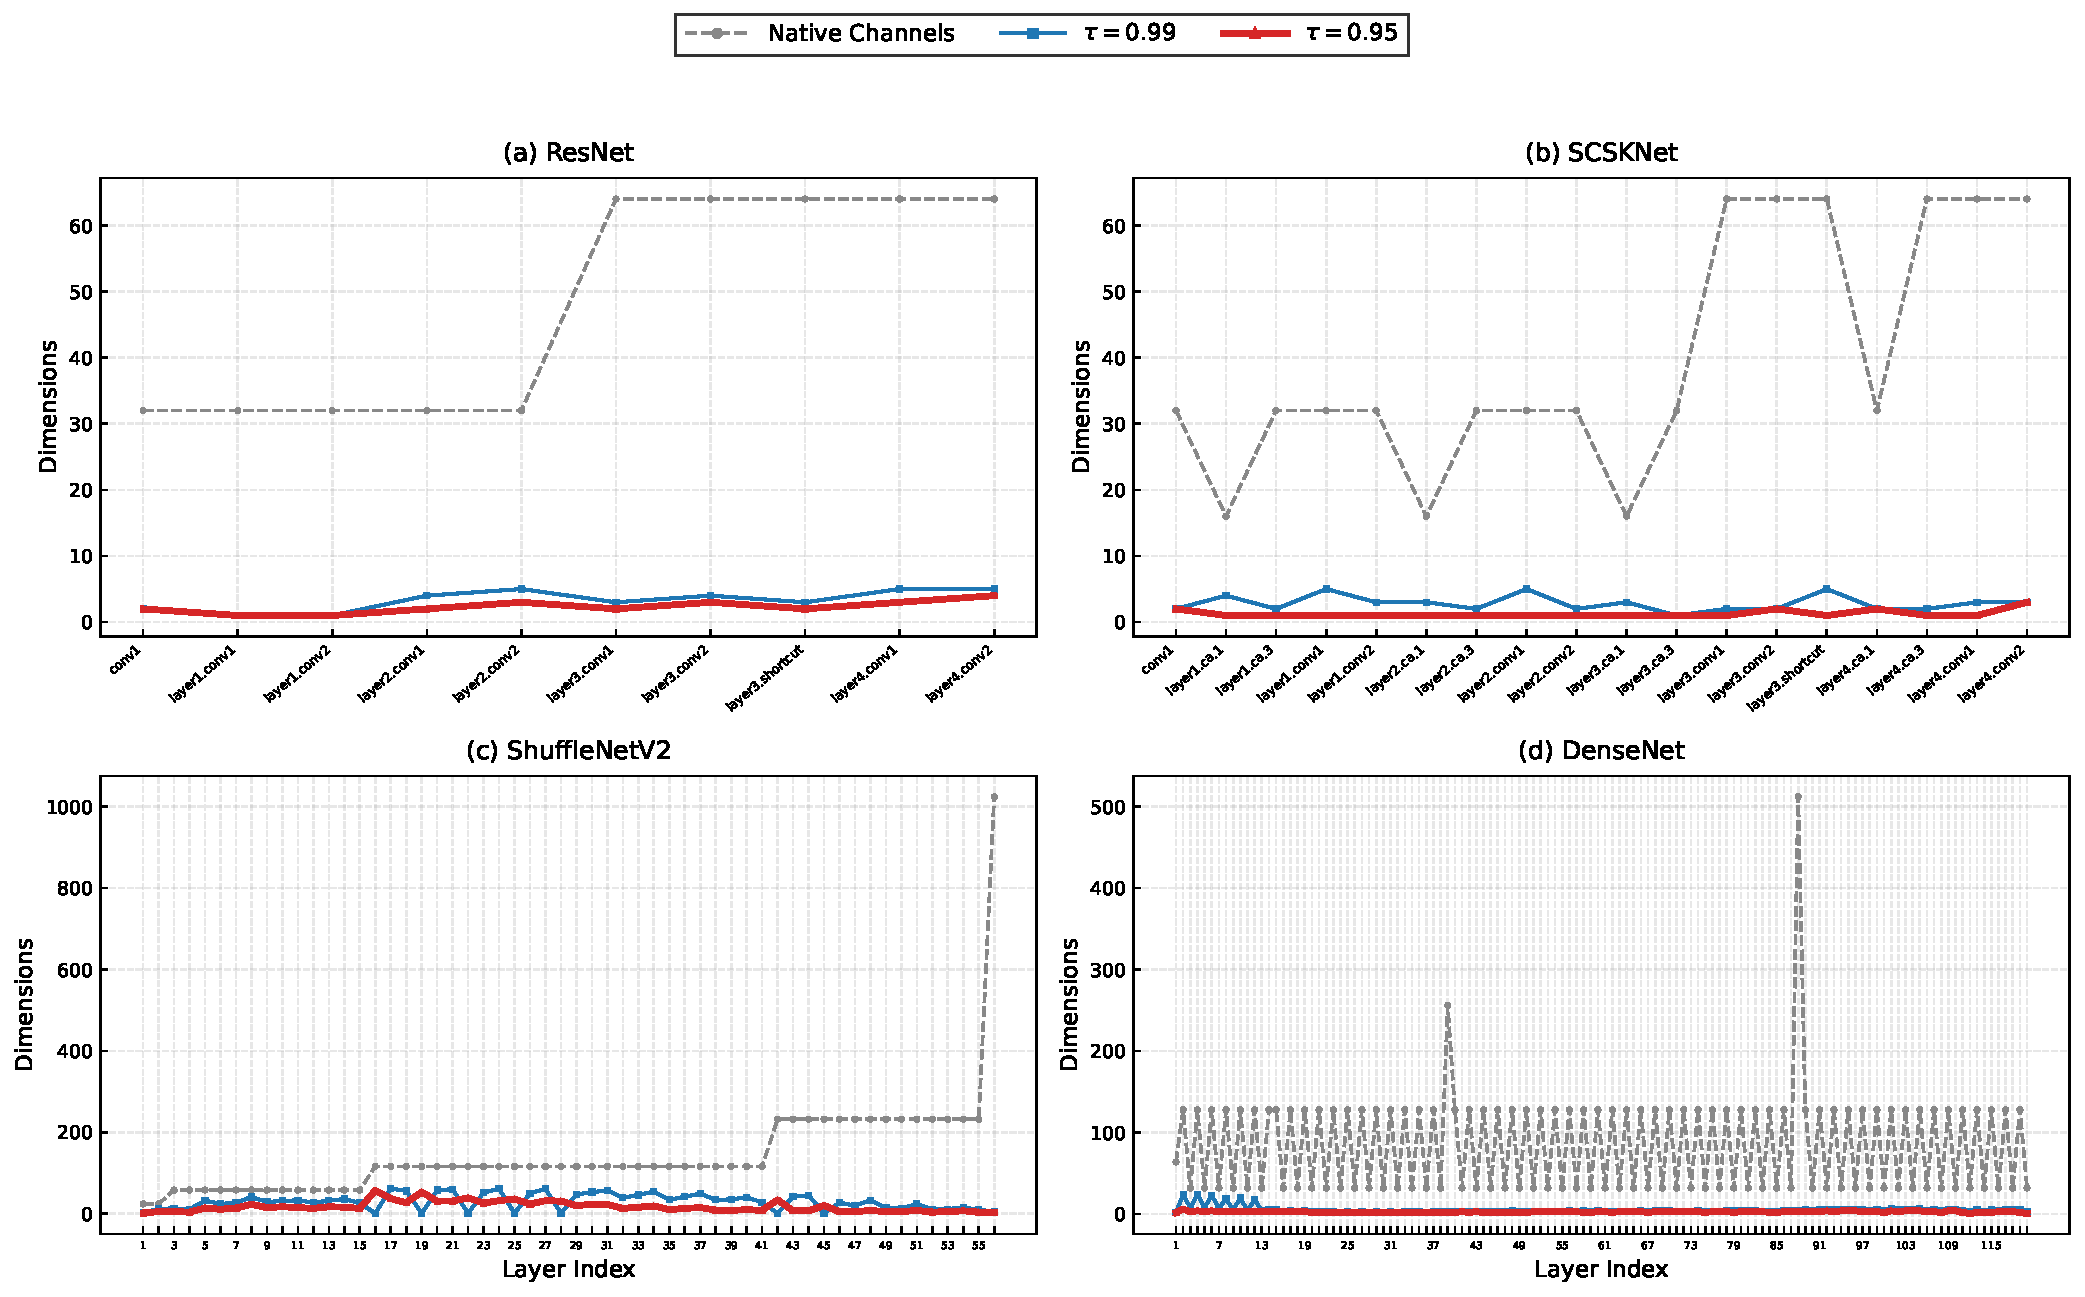
\includegraphics[width=0.95\linewidth]{figures/pca_comparison_four_networks.pdf}
    \caption{Per-layer PCA channel diagnosis on a trained Net.}
    \label{fig:pca_diagnosis}
\end{figure}

\subsection{Per-Layer PCA Diagnosis and Structural Redundancy}
\label{subsec:pca_diagnosis_visualization}

Prior to evaluating the global compression performance, we perform a granular analysis on the layer-wise energy spectra of the trained teacher networks to empirically substantiate the existence of structural redundancy. Fig.~\ref{fig:pca_diagnosis} illustrates the diagnostic results for the representative ResNet18 architecture under two distinct energy preservation thresholds, namely $\tau = 0.95$ and $\tau = 0.99$. 


\subsection{Distillation Across Different Network Families}

\begin{table*}[!t]
\caption{Comprehensive performance analysis: Complexity, Accuracy across Sub-scenarios, and Hardware Throughput.}
\label{tab:final_merged_complete}
\centering
\scriptsize 
\setlength{\tabcolsep}{2.8pt} % 保持紧凑的 23 列布局
\begin{tabular}{l|c|c|c|c|ccc|ccc|cc|cc|cc|ccc|ccc}
\toprule
\multirow{3}{*}{\textbf{Model}} & \multirow{3}{*}{\textbf{Type}} & \multirow{3}{*}{\textbf{Size}} & \multirow{3}{*}{\textbf{Params}} & \multirow{3}{*}{\textbf{FLOPs}} & \multicolumn{12}{c|}{\textbf{Accuracy (\%) Across Scenarios \& Sub-scenarios}} & \multicolumn{3}{c|}{\textbf{Jetson Nano}} & \multicolumn{3}{c}{\textbf{RTX 4090}} \\
\cmidrule(lr){6-17} \cmidrule(lr){18-20} \cmidrule(lr){21-23}
& & & & & \multicolumn{3}{c|}{\textbf{LOS}} & \multicolumn{3}{c|}{\textbf{NLOS}} & \multicolumn{2}{c|}{\textbf{Walk}} & \multicolumn{2}{c|}{\textbf{Mobile}} & \multicolumn{2}{c|}{\textbf{Antenna}} & \textbf{Feat.} & \textbf{Total} & \textbf{FPS} & \textbf{Feat.} & \textbf{Total} & \textbf{FPS} \\
\cmidrule(lr){6-8} \cmidrule(lr){9-11} \cmidrule(lr){12-13} \cmidrule(lr){14-15} \cmidrule(lr){16-17} \cmidrule(lr){18-20} \cmidrule(lr){21-23}
& & & & & \textbf{A} & \textbf{B} & \textbf{C} & \textbf{D} & \textbf{E} & \textbf{F} & \textbf{B} & \textbf{F} & \textbf{Off.} & \textbf{Meet.} & \textbf{B} & \textbf{F} & \textbf{ms} & \textbf{ms} & \textbf{1/s} & \textbf{$\mu$s} & \textbf{$\mu$s} & \textbf{1/s} \\
\midrule
\multirow{2}{*}{ResNet18} & Teacher & 802.32 KB & 203.26K & 268.12M & 99.7 & 98.5 & \textbf{99.8} & \textbf{100} & 62.5 & 98.5 & 92.6 & 98.9 & \textbf{86.4} & \textbf{88.8} & \textbf{99.2} & \textbf{90.2} & 4.45 & 33.36 & \fpeval{round(1000/(33.36),0)}  
& 94.3 & 166.0 & \fpeval{round(1000/(166.0),0)}K \\
& Student & 43.28 KB & 8.50K & 13.04M & \textbf{99.8} & \textbf{99.4} & 96.4 & 99.4 & \textbf{84.6} & \textbf{99.7} & \textbf{99.9} & \textbf{99.4} & 85.0 & 88.3 & 95.8 & 75.0 & 1.19 & 1.60 & \fpeval{round(1000/(1.60),0)} & 19.9 & 63.1 & \fpeval{round(1000/(63.1),0)}K \\
\midrule
\multirow{2}{*}{SCSKNet} & Teacher & 837.76 KB & 210.67K & 268.38M & \textbf{97.5} & \textbf{91.1} & \textbf{99.8} & \textbf{97.2} & \textbf{86.7} & \textbf{99.9} & \textbf{99.4} & \textbf{99.6} & \textbf{83.8} & 92.2 & \textbf{99.1} & 89.5 & 4.77 & 24.66 & \fpeval{round(1000/(24.66),0)} & 97.1 & 165.3 & \fpeval{round(1000/(165.3),0)}K \\
& Student & 33.51 KB & 4.95K & 7.25M & 95.3 & 88.2 & 99.1 & \textbf{97.2} & 79.7 & \textbf{99.9} & 93.4 & \textbf{99.6} & 80.8 & \textbf{95.0} & 97.6 & \textbf{91.3} & 0.89 & 1.31 & \fpeval{round(1000/(1.31),0)} & 16.7 & 58.6 & \fpeval{round(1000/(58.6),0)}K \\
\midrule
\multirow{2}{*}{ShuffleNet} & Teacher & 7124.85 KB & 1777.97K & 21.89M & 92.3 & 82.4 & 89.8 & 91.8 & 52.3 & \textbf{98.1} & 86.4 & \textbf{96.0} & 74.2 & \textbf{92.6} & 79.2 & \textbf{84.4} & 9.99 & 29.31 & \fpeval{round(1000/(29.31),0)} & 242.6 & 313.3 & \fpeval{round(1000/(313.3),0)}K \\
& Student & 294.85 KB & 42.74K & 1.19M & \textbf{95.8} & \textbf{93.1} & \textbf{89.9} & \textbf{92.7} & \textbf{68.1} & 96.3 & \textbf{94.8} & 93.8 & \textbf{79.0} & 88.2 & \textbf{88.9} & 83.6 & 0.77 & 1.08 & \fpeval{round(1000/(1.08),0)} & 42.3 & 84.6 & \fpeval{round(1000/(84.6),0)}K \\
\midrule
\multirow{2}{*}{DenseNet} & Teacher & 29768.69 KB & 7472.38K & 366.07M & 89.8 & 77.6 & 89.3 & 90.2 & 51.2 & 98.6 & 82.2 & 93.6 & 83.2 & 93.2 & 89.3 & \textbf{89.8} & 1.82 & 19.30 & \fpeval{round(1000/(19.30),0)} & 54.8 & 121.5 & \fpeval{round(1000/(121.5),0)}K \\
& Student & 144.51 KB & 8.96K & 1.60M & \textbf{90.0} & \textbf{78.6} & \textbf{89.6} & \textbf{92.2} & \textbf{60.4} & \textbf{99.7} & \textbf{84.4} & \textbf{96.0} & \textbf{85.6} & \textbf{98.5} & \textbf{89.8} & 88.2 & 0.69 & 1.01 & \fpeval{round(1000/(1.01),0)} & 49.7 & 92.4 & \fpeval{round(1000/(92.4),0)}K \\
\bottomrule
\end{tabular}

\begin{tablenotes}
\footnotesize
\item[*] Note: 'Off.' and 'Meet.' denote Office and Meeting settings. 'Feat.' represents the backbone feature extraction time, and 'Total' denotes the end-to-end latency including template matching classification.
\end{tablenotes}
\end{table*}

Table~\ref{tab:final_merged_complete} reports the comprehensive evaluation of the proposed pipeline across four diverse network architectures.

The ResNet18 teacher--student pair represents the canonical case where the teacher is well-trained.
The student reduces the parameter count from 203.26K to 8.50K (23.9$\times$ compression) and FLOPs from 268.12M to 13.04M (20.6$\times$ reduction), while maintaining competitive accuracy across all scenarios.
On LOS channels A and C, the student achieves 99.8\% and 96.4\% respectively, closely tracking the teacher's 99.7\% and 99.8\%.
Notably, the student surpasses the teacher on the NLOS E channel (84.6\% vs.\ 62.5\%) and on Walk B (99.9\% vs.\ 92.6\%), suggesting that the PCA-derived compact architecture is less prone to overfitting under channel degradation.
The student model occupies only 43.28~KB of storage, making it suitable for deployment on the most memory-constrained edge devices.

The remaining three architectures reveal a consistently recurring phenomenon: the distilled student outperforms its own teacher across a majority of test scenarios, often by substantial margins, despite operating at a fraction of the parameter budget.
The SCSKNet student reduces parameters by 42.6$\times$ (210.67K to 4.95K) yet achieves higher accuracy on the NLOS F channel (99.9\% tie) and on Mobile Meeting (95.0\% vs.\ 92.2\%).
The ShuffleNet student, at 42.74K parameters (41.6$\times$ compression), exceeds the teacher on 8 of the 12 evaluated scenarios, with the most pronounced gains on LOS B (93.1\% vs.\ 82.4\%, $+$10.7\%) and Walk B (94.8\% vs.\ 86.4\%, $+$8.4\%).
The DenseNet student achieves the most dramatic compression---from 7,472.38K to 8.96K parameters (834$\times$) and from 366.07M to 1.60M FLOPs (228.8$\times$)---while outperforming the teacher on 11 of the 12 scenarios, including NLOS D (92.2\% vs.\ 90.2\%) and Mobile Meeting (98.5\% vs.\ 93.2\%).

The empirical superiority of the student over its teacher stems from a dual purification mechanism. First, although the teacher networks—trained under severe SNR augmentations or early termination—exhibit non-trivial manifest noise under direct KNN evaluation, they still encode underlying structural inter-device similarities. Second, the PCA projection onto the $d_s$-dimensional subspace acts as an analytical filter, systematically discarding perturbation-dominated dimensions while isolating the dominant variance directions. By optimizing against these structurally filtered soft labels, the student network successfully bypasses the teacher's original empirical noise, yielding a more robust and purified representation.

\subsection{Iterative Distillation and Progressive Compression}

Fig.~\ref{fig:iterative} and Table~\ref{tab:iterative_trace} present the iterative distillation trajectory for ResNet across early rounds. Round 1 reduces parameters from 203.3K to 13.8K ($14.7\times$) while yielding even better generalization, with accuracy boosting to 84.6\% in NLOS-E. Round 2 further compresses the network to 3.0K parameters ($67.2\times$), maintaining acceptable performance (e.g., 97.05\% in NLOS-D) within the threshold $\delta = 20\%$. Though Round 3 approaches the information-theoretic minimum with 1.4K parameters, it still sustains a reasonable 92.70\% accuracy in NLOS-D, before the structural capacity completely collapses in Round 4.

\begin{figure}[t]
    \centering
    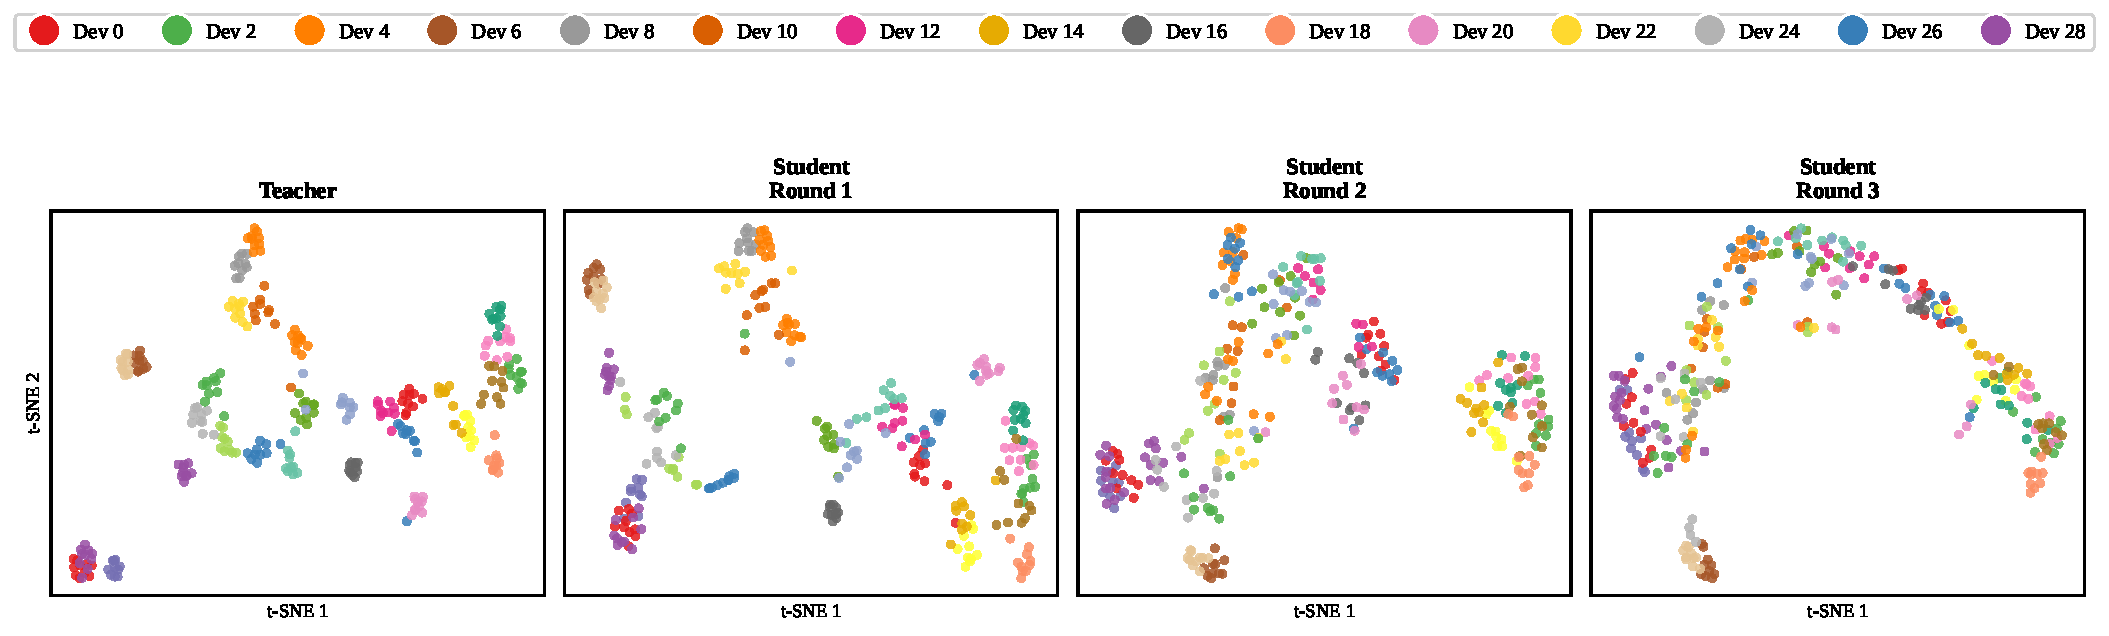
\includegraphics[width=0.95\linewidth]{figures/feature_visualization.pdf}
    \caption{Iterative distillation on ResNet across three rounds.}
    \label{fig:iterative}
\end{figure}

\begin{table}[t]
\caption{Per-layer PCA effective dimensions across iterative distillation rounds on ResNet.}
\label{tab:iterative_trace}
\centering
\footnotesize
\setlength{\tabcolsep}{5.5pt} % 优化间距，使多行表头排版更紧凑
\begin{tabular}{l|c|r|c|c|c}
\toprule
\textbf{Round} & \textbf{Channel Config} & \textbf{Params} & \textbf{LOS} & \textbf{NLOS} & \textbf{Walk} \\
& $[c_1, c_2, c_3, c_4, c_5]$ & & \textbf{-A} & \textbf{-D} & \textbf{-F} \\
\midrule
Teacher & [32, 32, 32, 64, 64] & 203,264 & 99.70 & 100.00 & 98.90 \\
Round 1 & [10, 12, 13, 19, 7]  & 13,784  & 99.80 & 99.40  & 99.40 \\
Round 2 & [8, 9, 4, 4, 4]       & 3,024   & 96.95 & 97.05  & 90.85 \\
Round 3 & [5, 6, 3, 2, 2]       & 1,364   & 96.00 & 92.70  & 96.85 \\
\bottomrule
\end{tabular}
\vspace{2pt}
\begin{tablenotes}
\footnotesize
\item[*] Note: LOS-A, NLOS-D, and Walk-F represent static line-of-sight, complex non-line-of-sight, and dynamic walking environments, respectively.
\end{tablenotes}
\end{table}

\subsection{Inference Latency on Edge Platforms}

To evaluate the real-time capability of the PCA-derived student networks, we measure inference latency, decomposing end-to-end latency into feature extraction and classification.
Results are reported in the rightmost columns of Table~\ref{tab:final_merged_complete}.

On the Jetson Nano, the ResNet18 teacher backbone requires 4.45~ms for feature extraction and 33.36~ms end-to-end (30~FPS), making it unsuitable for real-time per-packet authentication.
In contrast, all student backbones complete feature extraction in under 1.2~ms, with end-to-end latency ranging from 0.69~ms (DenseNet) to 1.60~ms (ResNet18), corresponding to 625--990~FPS on the same constrained hardware---a throughput that exceeds typical LoRa packet rates by a wide margin.

On the RTX~4090, the student backbones execute feature extraction within 16.7--49.7~$\mu$s per inference.
With PCA-accelerated classification, end-to-end throughput reaches 10,800--17,000~FPS across all student networks.
These results confirm that the proposed automated pipeline produces models that are not only parameter- and storage-efficient, but also latency-optimal for real-time edge RFFI deployment across heterogeneous hardware platforms.


\section{Conclusion}
\label{sec:conclusion}
This paper presents an automated lightweight RFFI pipeline that integrates PCA-driven channel diagnosis, structural pruning with random reinitialization, and self-distillation via PCA-aligned KL divergence.
By deriving per-layer channel budgets from the PCA energy spectrum of trained networks, the pipeline eliminates manual architecture design and replaces heuristic width multipliers with a data-driven criterion.
Self-distillation enables randomly-initialized compact networks to recover teacher-level discriminability, and we demonstrate that distillation additionally serves as a representation purification mechanism: students of undertrained teachers consistently outperform their teachers.
An iterative extension provides accuracy-bounded progressive compression, naturally converging to the channel-level information-theoretic floor.
Experiments across five diverse architectures on a real-world LoRa dataset demonstrate 14--834$\times$ parameter compression with minimal accuracy degradation, and edge deployment on an NVIDIA Jetson Nano achieves over 600~FPS inference throughput.
This work provides a practical, fully automated path toward deploying secure, low-latency RFFI systems on resource-constrained edge platforms without sacrificing performance.


\bibliographystyle{IEEEtran}
\bibliography{references}
\end{document}
